\section*{The repair layers}

To ensure that the neural network output respects the problem constraints, the paper proposes to add a sigmoid, and two repair layers to the end of the network. the sigmoid ensures that the generator output limits are respected, the first layer ensures that the power balance constraint is respected, and the second layer ensures that the reserve requirement is respected. in the paper it is shown that if there is a feasible solution, the repair layers will output a feasible solution.

\begin{figure}[ht]
    \centering
    \includegraphics[width=0.85\linewidth]{figs/repair_layers.pdf}
\end{figure}

The power balance repair layer $\mathcal{P}$ takes as input an initial dispatch vector $\pg \in \hypercube$ and outputs a dispatch vector $\mathbf{\tilde{p}}$ that also satisfies the power balance constraint.

\begin{figure}[ht]
    \centering
    \resizebox{0.42\columnwidth}{!}{
    \begin{tikzpicture}[x=2cm,y=2cm]
        % X Axis
        \draw[black,-stealth] (-0.1, 0.0) -- (1.25, 0.0);
        \node[below] at (1.25, 0.0) {\footnotesize $p_{1}$};
        % Y axis
        \draw[black,-stealth] (0.0, -0.1) -- (0.0, 1.25);
        \node[left] at (0.0, 1.25) {\footnotesize $p_{2}$};
        
        % Unit hypercube
        \draw[black] (0,0) -- (0, 1) -- (1,1) -- (1,0) -- cycle;
        
        % Power balance constraint
        \draw[red,line width=1pt] (0.1, 1.1) -- (1.1, 0.1);
        \node[right, color=red] at (0.1, 1.2) {\footnotesize $\mathbf{e}^{\top}\pg = D$};
        
        % Max output
        \node[draw=blue, fill=blue, inner sep=0pt,minimum size=3pt] (p_bar) at (1.00, 1.00) {};
        % Prediction
        \node[diamond,draw=blue, fill=blue, inner sep=0pt,minimum size=3pt] (p_hat) at (0.30, 0.30) {};
        \node[left] at (0.3, 0.3) {\footnotesize $\pg$};
        % Feasible point
        \node[circle,draw=blue, fill=blue, inner sep=0pt,minimum size=3pt] (p_til) at (0.6, 0.6) {};
        \node[right] at (0.65, 0.6) {\footnotesize $\mathbf{{\tilde{p}}}$};
        
        % Proportional response visual
        \draw[black,-stealth] (p_hat) -- (p_til);
        \draw[black,densely dotted] (p_til) -- (p_bar);
    \end{tikzpicture}}
    \hfill
    \resizebox{0.42\columnwidth}{!}{
    \begin{tikzpicture}[x=2cm,y=2cm]
        % X Axis
        \draw[black,-stealth] (-0.1, 0.0) -- (1.25, 0.0);
        \node[below] at (1.25, 0.0) {\footnotesize $p_{1}$};
        % Y axis
        \draw[black,-stealth] (0.0, -0.1) -- (0.0, 1.25);
        \node[left] at (0.0, 1.25) {\footnotesize $p_{2}$};
        
        % Unit hypercube
        \draw[black] (0,0) -- (0, 1) -- (1,1) -- (1,0) -- cycle;
        
        % Power balance constraint
        \draw[red,line width=1pt] (0.1, 1.1) -- (1.1, 0.1);
        \node[right, color=red] at (0.1, 1.2) {\footnotesize $\mathbf{e}^{\top}\pg = D$};
        
        % Min output
        \node[draw=blue, fill=blue, inner sep=0pt,minimum size=3pt] (p_bar) at (0.00, 0.00) {};
        % Prediction
        \node[diamond,draw=blue, fill=blue, inner sep=0pt,minimum size=3pt] (p_hat) at (0.80, 0.80) {};
        \node[right] at (0.8, 0.8) {\footnotesize $\pg$};
        % Feasible point
        \node[circle,draw=blue, fill=blue, inner sep=0pt,minimum size=3pt] (p_til) at (0.6, 0.6) {};
        \node[left] at (0.58, 0.58) {\footnotesize $\mathbf{{\tilde{p}}}$};
        
        % Proportional response visual
        \draw[black,-stealth] (p_hat) -- (p_til);
        \draw[black,densely dotted] (p_til) -- (p_bar);
    \end{tikzpicture}}
    \hfill\\
    \caption{%
        Illustration of the power balance layer with input $\pg$ and output $\mathbf{\tilde{p}}$.
        Left: $\mathbf{e}^{\top}\pg \, {<} \, D$ (energy shortage) and generators' dispatches are increased.
        Right: $\mathbf{e}^{\top}\pg \, {>} \, D$ (energy surplus) and generators' dispatches are decreased.
    }
    \label{fig:feasibility_layer:hypersimplex}
\end{figure}


the output is given by:

\begin{align*}
    \mathcal{P}(\pg) &= \begin{cases}
        (1 - \eta^{\uparrow}) \pg + \eta^{\uparrow} \pgmax & \text{if } \mathbf{e}^{\top} \pg < \mathbf{e}^{\top} \pd \\
        (1 - \eta^{\downarrow}) \pg + \eta^{\downarrow} \mathbf{0} & \text{if } \mathbf{e}^{\top} \pg > \mathbf{e}^{\top} \pd
    \end{cases} \\
    \eta^{\uparrow} &= \frac{\mathbf{e}^{\top} \pd - \mathbf{e}^{\top} \pg}{\mathbf{e}^{\top} \pgmax - \mathbf{e}^{\top} \pg}, \quad
    \eta^{\downarrow} = \frac{\mathbf{e}^{\top} \pg - \mathbf{e}^{\top} \pd}{\mathbf{e}^{\top} \pg - \mathbf{e}^{\top} \mathbf{0}}
\end{align*}

The reserve repair layer $\mathcal{R}$ takes as input an initial dispatch vector $\pg \in \hypersimplex{D}$ and outputs a dispatch vector $\mathbf{\tilde{p}}$ that also satisfies the reserve requirement.

\begin{figure}[ht]
    \centering
    \resizebox{0.6\columnwidth}{!}{
    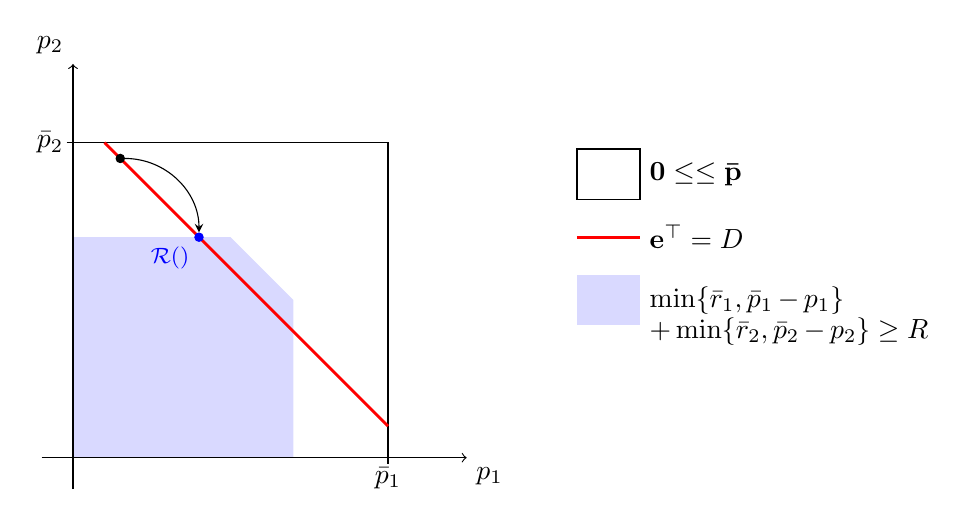
\begin{tikzpicture}[x=4cm,y=4cm]
        % X Axis
        \draw[black,->] (-0.1, 0.0) -- (1.25, 0.0);
        \node[below right] at (1.25, 0.0) {$p_{1}$};
            \draw[black] (1, -0.02) -- (1, 0.02);
            \node[below] at (1, 0.0) {$\bar{p}_{1}$};
        
        % Y axis
        \draw[black,->] (0.0, -0.1) -- (0.0, 1.25);
        \node[above left] at (0.0, 1.25) {$p_{2}$};
            \draw[black] (-0.02, 1) -- (+0.02, 1);
            \node[left] at (0, 1) {$\bar{p}_{2}$};
            
        % Reserve feasibility domain
        \fill[blue!50!white, fill opacity=0.3] (0,0) -- (0,0.7) -- (0.5, 0.7) -- (0.7, 0.5) -- (0.7, 0.0) -- cycle;
        
        % Domain of p1, p2
        \draw[black] (0,0) -- (0, 1) -- (1,1) -- (1,0) -- cycle;
        
        % Power balance constraint
        \draw[red,line width=1pt] (0.1, 1.0) -- (1.0, 0.1);
        
        % Infeasible prediction
        \node[circle,draw=black, fill=black, inner sep=0pt,minimum size=3pt] (phat_a) at (0.15, 0.95) {};
        \node[below left] at (0.15, 0.95) {\footnotesize $\pg$};
        
        % Feasible points of interest
        \node[circle,draw=blue, fill=blue, inner sep=0pt,minimum size=3pt] (pfeas1) at (0.4, 0.7) {};
        \node[below left, blue] at (0.4, 0.7) {\footnotesize $\mathcal{R}(\pg)$};
        
        \draw[-stealth] (phat_a.east) to [out=0,in=90] (pfeas1.north);
        
        % Legend
            % Domain of pg
            \draw[black] (1.6, 0.98) -- (1.8, 0.98) -- (1.8, 0.82) -- (1.6, 0.82) -- cycle;
            \node[right] at (1.8, 0.9) {$\mathbf{0} \leq \pg \leq \mathbf{\bar{p}}$};
            % Power Balance
            \draw[red, line width=1pt] (1.6, 0.7) -- (1.8, 0.7);
            \node[right] at (1.8, 0.7) {$\mathbf{e}^{\top} \pg = D$};
            % Reserve feasibility
            \fill[blue!50!white, fill opacity=0.3] (1.6, 0.58) -- (1.8, 0.58) -- (1.8, 0.42) -- (1.6, 0.42) -- cycle;
            \node[right] at (1.8, 0.5) {$\min\{\bar{r}_{1}, \bar{p}_{1} \, {-} \, p_{1}\}$};
            \node[right] at (1.8, 0.4) {$+\min\{\bar{r}_{2}, \bar{p}_{2} \, {-} \, p_{2}\} \geq R$};
    \end{tikzpicture}
    }
    \caption{Illustration of the reserve feasibility layer for $\mathbf{\bar{p}} {=} (1, 1)$, $\mathbf{\bar{r}}{=}(0.5, 0.5)$, $D {=} 1.1$, $R{=}0.8$ and the initial prediction $\pg {=} (0.15, 0.95)$. The recovered feasible dispatch is $\mathbf{\tilde{p}} {=} (0.4, 0.7)$.}
    \label{fig:feasibility_recovery:reserve}
\end{figure}


the output is given by the following algorithm:
\begin{algorithm}[t]
    \caption{Reserve Repair Layer}
    \label{alg:FFR:reserves}
    \begin{algorithmic}[1]
        \REQUIRE Initial prediction $\pg \in \hypersimplex{D}$, maximum limits $\mathbf{\bar{p}}, \mathbf{\bar{r}}$, reserve requirement $R$
        \STATE $\Delta_{R} \gets R - \sum_{g} \min \{ \bar{r}_{g}, \bar{p}_{g} - p_{g} \}$
        \STATE $\mathcal{G}^{\uparrow} \gets \left\{ g \ \middle| \ p_{g} \leq \bar{p}_{g} - \bar{r}_{g} \right\}$
        \STATE $\mathcal{G}^{\downarrow} \gets \left\{ g \ \middle| \  p_{g} > \bar{p}_{g} - \bar{r}_{g} \right\}$
        \STATE $\Delta^{\uparrow} \gets \sum_{g \in \mathcal{G}^{\uparrow}} (\bar{p}_{g} - \bar{r}_{g}) - p_{g}$
        \STATE $\Delta^{\downarrow} \gets \sum_{g \in \mathcal{G}^{\downarrow}} p_{g} - (\bar{p}_{g} - \bar{r}_{g})$
        \STATE $\Delta \gets \max(0, \min(\Delta_{R}, \Delta^{\uparrow}, \Delta^{\downarrow}))$
        \STATE $\alpha^{\uparrow} \gets \Delta / \Delta^{\uparrow}$, $\alpha^{\downarrow} \gets \Delta / \Delta^{\downarrow}$, \label{alg:FFR:proportional_response_weigths}
        \STATE Energy dispatch adjustment
            \begin{align*}
                \tilde{p}_{g} &= \left\{
                    \begin{array}{ll}
                        (1 - \alpha^{\uparrow}) p_{g} + \alpha^{\uparrow} (\bar{p}_{g} - \bar{r}_{g}) & \forall g \in \mathcal{G}^{\uparrow} \\
                        (1 - \alpha^{\downarrow}) p_{g} + \alpha^{\downarrow} (\bar{p}_{g} - \bar{r}_{g}) & \forall g \in \mathcal{G}^{\downarrow}
                    \end{array}
                \right.
            \end{align*}
            \label{alg:FFR:proportional_response}
        \STATE \textbf{return} $\mathcal{R}(\pg) = \mathbf{\tilde{p}}$
    \end{algorithmic}
\end{algorithm}

